% !TeX spellcheck = en_US
\documentclass{bioinfo}

\usepackage{hyperref} \usepackage{tikz} \usetikzlibrary{graphs}

\let\proglang=\textsf

\copyrightyear{2017} \pubyear{2017}

\begin{document} \firstpage{1}
\title[RDML]{Enabling reproducible real-time quantitative PCR research: the RDML package}
\author[Blagodatskikh \textit{et~al}]{Stefan R\"{o}diger\,$^{1}$, Micha\l{} Burdukiewicz\,$^{2}$, Andrej-Nikolai Spiess\,$^{3}$ and Konstantin Blagodatskikh\,$^{4}$\footnote{to whom correspondence should be addressed}} 

\address{
$^{1}$Institute of Biotechnology, Brandenburg University of Technology Cottbus--Senftenberg, Senftenberg, Germany\\ 
$^{2}$Department of Genomics, Faculty of Biotechnology, University of Wroc\l{}aw, Wroc\l{}aw\\
$^{3}$University Medical Center Hamburg-Eppendorf, Hamburg, Germany\\
$^{4}$Evrogen JSC, Moscow, Russia\\ 
}
\history{Received on XXXXX; revised on XXXXX; accepted on XXXXX}

\editor{Associate Editor: XXXXXXX}
\maketitle

\begin{abstract}
\section{Motivation:} Reproducible research is essential in science. 
Part of this are open standards for data exchange, which preserve 
the set-up and output of experiments in defined schemes. The Real-time PCR 
Data Markup Language (RDML) is a recommended standard of the Minimum Information 
for Publication of Quantitative Real-Time PCR Experiments (MIQE) guidelines. 
Even though selected software products of qPCR instruments export RDML data, 
there is no tool designed for working with RDML data in a sophisticated 
environment for statistical bioinformatics.
\section{Results:} We developed the cross-platform open source \textit{RDML} 
package for the statistical computing language \textbf{R}. \textit{RDML} is 
compliment to RDML~$\geq$~v.~1.2 and provides functionality to (i) import RDML 
data; (ii) extract sample information (e.g., targets, concentration); (iii) 
transform data to various formats of the \textbf{R} environment; (iv) 
generate human readable experiment summaries; and (v) to create RDML files from 
user data. In addition, \textit{RDML} offers a graphical user interface to read, 
edit and create RDML files. We show that \textit{RDML} enables seamless analysis 
with other \textbf{R} packages.

\section{Availability:} \url{https://cran.r-project.org/package=RDML}. Source code: 
\url{https://github.com/kablag/RDML}. \section{Contact:} 
\href{k.blag@yandex.ru}{k.blag@yandex.ru} \end{abstract}


\section{Introduction}
Real-time quantitative PCR (qPCR) is one of the most widely applied methods in molecular 
biology, diagnostics and genetical testing. qPCR is well accepted since 
it is simple, accurate, reliable and reproducible \cite{pabinger_2014}. The 
Minimum Information for Publication of Quantitative Real-Time PCR Experiments (MIQE) were established to facilitate the comparison of experimental results obtained from qPCR 
\cite{huggett_2013}. There are at least twenty different qPCR cycler manufacturers. Such variety creates a broad selection to 
address specific market demands. The systems differ largely in the 
number of processable samples, number of detection channels and sample 
arrangement (e.g., plate, carousel). Moreover, the devices use different 
data processing methods and non-interchangeable storage formats (e.g., binary formats). 
Binary data formats and system specific formats often result in an undesired vendor 
lock-in. This diversification comes at a cost at the level of data 
exchange. Discrepancies in data processing hinders comparisons of PCR results 
obtained on different systems, and disparate storage formats prohibit the processing 
of raw data from one instrument in other systems. This is essentially contra-productive as data processing poses a 
challenge in qPCR data analysis \cite{bustin_reproducibility_2014, roediger2015r, 
spiess_impact_2014, spiess_system-specific_2016}.

The MIQE guidelines suggest Real-time PCR Data Markup Language (RDML) as the standard 
qPCR interchange data format \cite{rdml-ninja_2015}. RDML is a vendor 
independent and freely available file format. It is based on the 
eXtensible Markup Language (XML), which is commonly used in bioinformatics 
\cite{achard_xml_2001} to pass metadata and values between applications. 
Here, the storage and exchange of qPCR data is bidirectional. The RDML data standard 
contains the primary raw data acquired by the qPCR system, meta-information to 
understand the experimental setup (e.g., sample annotation, qPCR protocol, probe 
and primer sequences) and information to re-analyse the data 
\cite{lefever_rdml_2009}. Different vendors (see 
Supplement) and third-party software (e.g., \textit{Primer3Plus} 
\cite{untergasser_2007}, \textit{QPCR}, \textit{LinRegPCR}, \textit{qBase+}) 
\cite{pabinger_2014, rdml-ninja_2015} support the RDML format. Despite its openness, 
there exists no open source software capable of reading, processing and writing 
this format. Instead, users have to choose between programs from manufacturers of qPCR 
devices, which can use only their own generated files, or alternatively commercial software 
such as \textit{qbase+} \cite{pabinger_2014, rdml-ninja_2015}. Recently, 
Ruijter~\textit{et~al.} published the open-source desktop software 
\textit{RDML-Ninja}, which can visualize, edit and validate RDML files 
\cite{rdml-ninja_2015}. However, \textit{RDML-Ninja} cannot analyze qPCR 
data by sophisticated analysis pipelines, limiting its applications in 
customized high-throughput applications. Moreover, there is a need for a \textit{de novo} 
creation of RDML data in systems that do not 
support the RDML format (e.g., commercial systems, prototypes, point-of-care devices). 

The cross-platform statistical computing language \textbf{R} is the \textit{de facto} standard in applied 
statistical bioinformatics, provides comprehensive tool-sets for reproducible research \cite{leeper_archiving_2014, 
liu_r_2014, roediger2015r} and is suitable for standalone desktops or servers \cite{roediger2015r}. 
Although there are \textbf{R} packages for qPCR and melting 
curve analysis available \cite{pabinger_2014, ritz_qpcr_2008, 
roediger_RJ_2013, roediger2015chippcr}, it was not previously possible 
to seamlessly process RDML files.

The common strategy for data management in \textbf{R} is native formats such 
as \textbf{R} workspaces and objects \cite{roediger_rkward_2012}. However, 
the external application of these formats is limited with respect to the RDML format, 
a specifically tailored variant of XML. Hence, the principle of reproducible research 
is not warranted without a standard method of data import such as the \textit{RDML} 
package. Our software enables the application of qPCR-related \textbf{R} tools, as 
recently reviewed in \cite{pabinger_2014}, while working on RDML data directly 
derived from the qPCR system. To conclude, the \textit{RDML} package may 
serve as a foundation for other \textbf{R} packages hosted at Bioconductor 
\cite{gentleman_2004} and CRAN, as shown recently \cite{roediger2015r}.

Here, we describe the \textit{RDML} package, which 
allows to exchange RDML files ($\geq$~v.~1.1) and transform them to a human 
readable format. Up to version \textit{RDML} package 0.8-3, only RDML~v.~1.1 and 
file import was supported. Here, we present a considerably maturated version of 
the package, including a novel graphical user interface (GUI) to read, edit and create RDML files. The \textit{RDML} package is open-source, free to use, 
platform-independent, can be modified for specific tasks or other 
\textbf{R} packages, or even be integrated with work-flows of other programming 
languages. Although many qPCR instruments as well as software solutions are able 
to work with the RDML format, there is a need to make RDML available for the increasingly 
used \textbf{R} environment.

\section{Implementation}
The \textit{RDML} package is available at CRAN 
(\url{https://cran.r-project.org/package=RDML}) and the 
development version is hosted at GitHub (\url{https://github.com/kablag/RDML}) 
with facilities for bugs reports and feature requests. \textit{RDML} provides 
\emph{R6} classes, which corresponds to RDML~v.~1.2 input format types. 

\textbf{R} 
is a language with dynamic typing. This is helpful while scripting, but can lead 
to problematic debugging of more complicated workflows. \emph{R6} classes 
provide type-safe interfaces to set data without access to the inner structure of 
objects so that all imported data can be validated. This option is highly useful when 
creating packages at an intermediate level for other packages (e.g., such an
approach does not permit set type \emph{character} in place of type \emph{integer}, 
Supplementary Section S3.3). Furthermore, the inheritance of \emph{R6} objects 
unifies the structure of the package and streamlines the extending of its capabilities 
(since the whole package is written around a single base class). Although the main interaction 
is via the command line interface (CLI) to enable batch processing,we designed a graphical user
interface (\textbf{rdmlEdit}) based on the \textit{shiny} technology \cite{shiny_2016}. This GUI allows editing of RDML metadata and visualizing the raw, unprocessed fluorescence data
(Fig.~\ref{fig:02}). The RDML file format, coordinated by the RDML consortium (www.rdml.org/), is under continuous development. The \textit{RDML} 
package adheres to the changes and supports the current version RDML~v.~1.2. 
Central functionalities of the \textit{RDML} package encompass the read-in of RDML 
data files and the summary generation for RDML objects. The public methods of the main “RDML” class can be used 
to access and process the internally stored RDML data. These methods include:

\begin{itemize} 
\item \textbf{\$new()} -- creates a new RDML object, empty or from a specified RDML 
file (Supplementary Section S3.1 and S3.10-3.13);
\item \textbf{\$AsDendrogram()} -- plots the
structure of an RDML object as a dendrogram (Fig.~ \ref{fig:01} and Supplementary Section 
S3.1);
\item \textbf{\$AsTable()} -- represents the data contained in an RDML object (except 
fluorescence data) as a \textit{data.frame} (Supplementary Section S3.4);
\item \textbf{\$GetFData()} -- gets fluorescence data (Supplementary Section S3.5);
\item \textbf{\$SetFData()} -- sets fluorescence data to an RDML object (Supplementary Section S3.6); 
\item \textbf{\$AsXML()} – saves an RDML object as an RDML~v.~1.2 file (Supplementary Section S3.8).
\end{itemize}
In addition to working with existing RDML files, the package can create new RDML 
objects from qPCR data of systems that do not support the RDML format. To 
create an eligible RDML object, one has to provide fluorescence data and a minimal 
description of the experiment (Supplementary Section S3.10). Another unique feature of the \textit{RDML} 
package is the ability to merge several RDML files (experiments) into one single file with the 
\textbf{MergeRDMLs()} function and process it like a unit (Fig.~\ref{fig:01} and Supplementary Section 
S3.7). For example, one can combine the results of two runs with samples of one 
experiment or add calibration samples to a run with genes-of-interest.

\begin{figure}
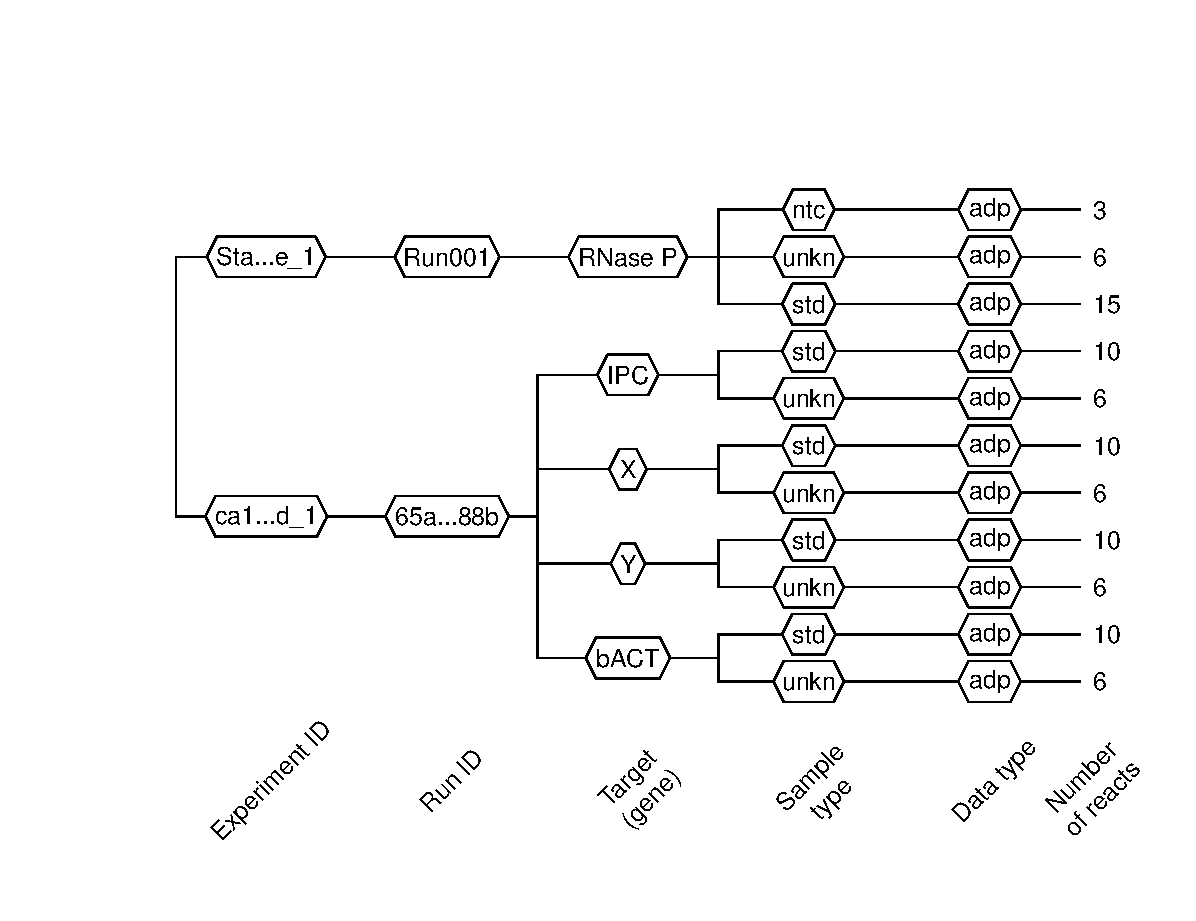
\includegraphics[width=0.5\textwidth]{as_dendrogram.eps}
\caption{Structure of an RDML object represented as a dendrogram via the 
	\textbf{\$AsDendrogram()} function. Two files 
	were loaded and merged into one object. As a result, two 
	experiments can be processed in one pipeline.}\label{fig:01}
\end{figure}
\begin{figure}
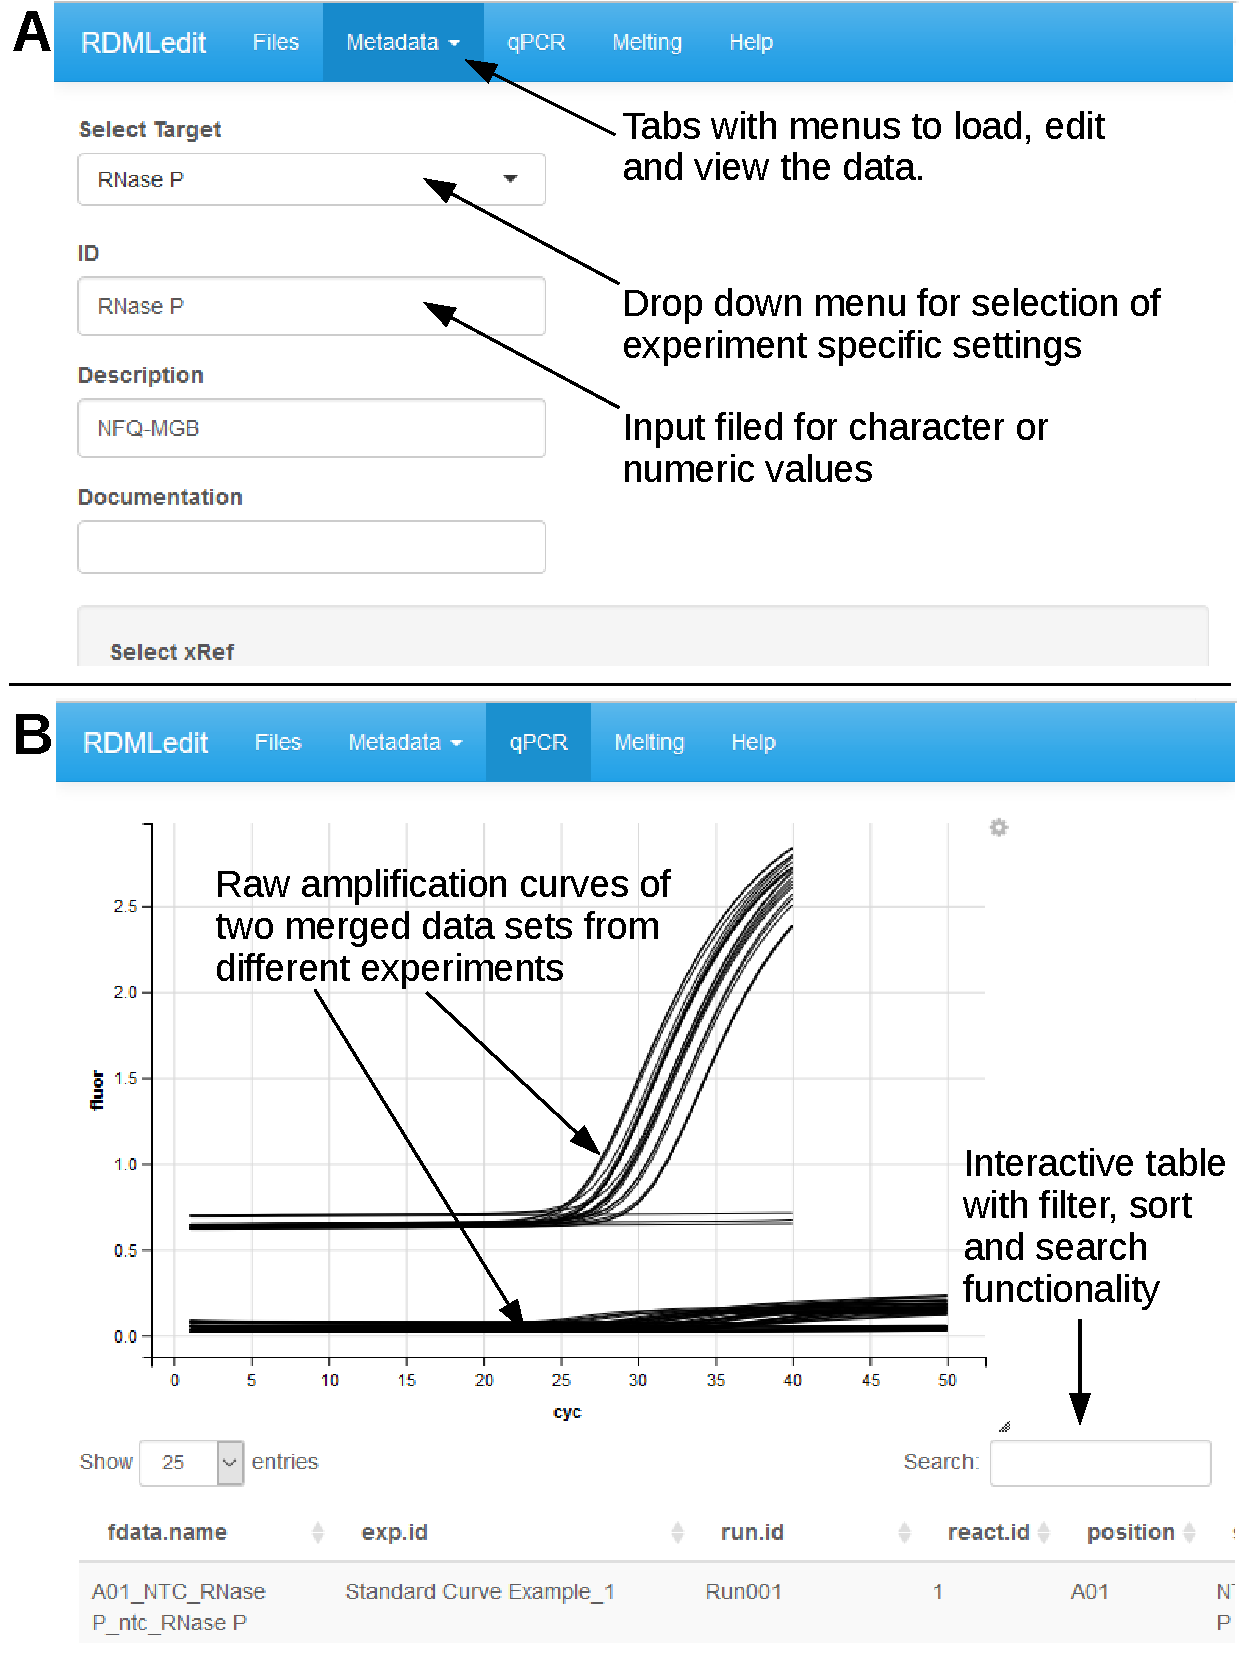
\includegraphics[width=0.5\textwidth]{figure_gui.pdf}
\caption{Working with RDML files in the \textbf{rdmlEdit} GUI. 
  	(A) The function \textbf{rdmlEdit()} invokes a shiny GUI which allows to 
	merge data, edit meta-data (e.g., - Target). (B) The GUI has tools to view the raw 
	data of the amplification (tab ``qPCR'') and melting curves (tab ``Melting Curves''). Both the plot and 
	the table are interactive with highlighting and filter features.}\label{fig:02}
\end{figure}

\section{Basic qPCR Analysis}

In contrast to other RDML software provides the \textit{RDML} package basic 
preprocessing and analysis capabilities including the Cq calculation based on 
the second derivative maximum method and cycle threshold method based on 
findings described in \cite{roediger_RJ_2013, roediger2015chippcr, 
spiess_impact_2014, spiess_system-specific_2016}. The intention is to give the 
user an overview of the data for quality control and experiment planning. It 
is recommended to the users of the \textit{RDML} package to evaluate their own 
analysis pipeline based on evidence based principles as described elsewhere 
\cite{ritz_qpcr_2008, roediger2015r}. In particular, the cycle threshold method 
is problematic \cite{spiess_impact_2014, spiess_system-specific_2016}. Other Cq 
methods were challenged too \cite{ruijter_evaluation_2013}.
The \textbf{rdmlEdit()} can be used to preview the raw data and to do some basic 
data mining. However, advanced steps like pooling of the different runs, 
visualization and processing (e.g., correction of interplate variance \cite{ruijter_removal_2015}, 
imputation of missing values \cite{mccall_non-detects_2014}) are important task. Such tasks can be performed 
independently in R via the programming language.

\section{Discussions and Conclusions}

The \textit{RDML} package for \textbf{R} imports and manipulates data 
from RDML~v.~1.1 and v.~1.2 format files and can create RDML~v.~1.2 files 
from user provided data. This package can be used as part of the qPCR 
processing workflow or for preliminary summaries of experiments. Due to the 
openness of the format, we anticipate that other scientific disciplines might 
benefit from this implementation. Data processed with the \textit{RDML} package 
can be subjected to further statistical analysis with dedicated algorithms to 
deal with non-detects \cite{mccall_non-detects_2014}, normalization 
\cite{perkins_readqpcr_2012} and expression analysis \cite{dvinge_htqpcr:_2009, matz_no_2013}.

Researchers often collect gene expression data from more than one laboratory and 
and are thus required to analyze and aggregate many data sets. Adaptable data 
management - also known as “adaptive informatics” - is relevant in cases where 
data from different omics approaches and assays (e.g., flow cytometry, digital 
PCR, NGS) need to be merged \cite{baker_quantitative_2012}. As RDML is based on 
XML, it is possible to converge the files with other formats such as HDF, 
\cite{millard_adaptive_2011} which is supported by \textbf{R} 
\cite{Fischer_HDF5}. This enables extended data storage and analysis, but also a 
higher level of experimental data management.

\section{Acknowledgements}
Grateful thanks belong to the \textbf{R} community and the RDML consortium.
\paragraph{Conflict of Interest\textcolon} none declared.

%\bibliographystyle{natbib}
%\bibliographystyle{achemnat}
%\bibliographystyle{plainnat}
%\bibliographystyle{abbrv}
%\bibliographystyle{bioinformatics}
%
\bibliographystyle{plain}
%
\bibliography{RDML}

\end{document}
